\documentclass[conference]{IEEEtran}

\usepackage[utf8]{inputenc}
\usepackage[T1]{fontenc}
\usepackage{silence}\WarningsOff[latexfont]

\usepackage{amsmath}

\RequirePackage{tikz}[2010/10/13]
\usetikzlibrary{arrows,automata,calc,intersections,patterns,decorations.pathmorphing,decorations.pathreplacing}

\usepackage{graphicx}
\usepackage{cite}
\usepackage{url}
\usepackage[caption=false,font=footnotesize]{subfig}
\usepackage[binary-units,per-mode=symbol]{siunitx}
\sisetup{list-final-separator = {, and }}
\usepackage{booktabs}
\usepackage{pifont}
\usepackage{microtype}
\usepackage{textcomp}
\usepackage[american]{babel}
\usepackage[noabbrev,capitalise]{cleveref}
\usepackage{xspace}
\usepackage{hyphenat}
\usepackage[draft,inline,nomargin,index]{fixme}
\fxsetup{theme=color}
\usepackage{grffile}
\usepackage{xfrac}
\usepackage{multirow}
\RequirePackage{xstring}
\RequirePackage{xparse}
\RequirePackage[index=true]{acro}

\NewDocumentCommand\acrodef{mO{#1}mG{}}{\DeclareAcronym{#1}{short={#2}, long={#3}, #4}}
\NewDocumentCommand\acused{m}{\acuse{#1}}

\usepackage{upquote}

\usepackage{tikz}
\usetikzlibrary{positioning,shapes,arrows}

\acrodef{DAG}{directed acyclic graph}
\acrodef{EM}{expectation–maximization}
\DeclareMathOperator*{\argmax}{arg\!\max}

\newcommand\Tstrut{\rule{0pt}{2.6ex}}         % = `top' strut
\newcommand\Bstrut{\rule[-0.9ex]{0pt}{0pt}}   % = `bottom' strut


\begin{document}

\title{Assignment 1 - Bayesian Networks}
\author{
	\IEEEauthorblockN{Davide Pedranz, Mat. number 189295}
	\texttt{davide.pedranz@studenti.unitn.it}
}

\maketitle

\begin{abstract}
Bayesian networks are powerful graphical probabilistic models widely used if various fields.
In this assignment, we compare some of the available algorithms to learn the structure of a Bayesian network from a dataset of samples.
\end{abstract}

\acresetall

% various sections
\section{Introduction}
\label{sec:introduction}

Bayesian networks are graphical statistical models that represent the joint probability distribution and conditional dependencies of a set of random variables via a \ac{DAG}.
They help to visualize the structure of the model in an intuitive way and allow all kinds of probabilistic inference on it.

A typical application of the Bayesian modelling is for diagnosis: given some clinical tests (observations), we want to estimate the probability of having some diseases (causes).
In general, Bayesian networks can be used for any kind probabilistic inference.
Common tasks are computing conditional independence between groups of random variables and computing the probability of a certain configuration given a set of observations.

Bayesian networks are usually build with the help of a domain expert, who knows some of the causality and independence relationships between the random variables, as well as some rough conditional probabilities of a random variables given its possible causes (the parents in the \ac{DAG}).

Given a network, there are algorithms to learn the model parameters from training data, or, if all parameters are given, tune them to better fit the data.
There are also algorithms to learn the structure of the network.
In this assignment, we focus on learning the structure of the network using different algorithms and comparing their performances on a given learning problem.
In particular, we use the \texttt{HUGIN Lite}\footnote{Available at: \url{http://www.hugin.com/index.php/hugin-lite/}} software to learn the structure of the network using two different algorithms:
\begin{itemize}
    \item NPC
    \item Greedy search-and-score
\end{itemize}
Moreover, we compare the results with a Naive Bayes structure.

\section{Learning problem}
\label{sec:learning-problem}

We want to understand the relationships of 6 given genes: \texttt{ATP2B4}, \texttt{NAP1L1}, \texttt{MDK}, \texttt{PCCB}, \texttt{MDS1}, \texttt{AML}.
Each gene can be active or inactive and can influence the status of the others.
We are interested in predicting the probability of gene \texttt{AML} to be active, given the status of the others.

First, we will learn a Bayesian network using one of the algorithms described in \cref{sec:introduction}.
Then, we will use the build in \ac{EM} algorithm to learn the model's parameters.
Finally, we will evaluate the network's performances on predicting gene \texttt{AML}.

We are given dataset that contains \num{72} complete examples of the \num{6} genes.
We will use \num{80}\% of them for the training and the remaining \num{20}\% for the test.
Given the small number of examples, we will use the k-fold cross validation technique (explained in \cref{sec:cross-validation}) to get more reliable results.

\section{k-fold cross validation}
\label{sec:cross-validation}

A typical approach to evaluate the performances of a supervised learning algorithm is to test its prediction of on some labeled test data.
To do that, the examples are divided in two parts: a training set, used to train the learner, and a validation test, used to evaluate its performances.
The learner never sees the test set before, so the results tells how good the learner will generalize on future data.

A common setting is to use $70 - 80\%$ of the data for the training and the remaining $20 - 30\%$ for the test.
This works fine as long as the available dataset is big enough, but the learner has problems if the dataset is small, since this further reduces the number of available examples.
In fact, the learner tends not to generalize properly if trained with insufficient examples.

k-fold cross validation is a technique that tries to reduce this problem.
The dataset is randomly partitioned in k equal sized sets.
Instead of just one, k different learners are trained, each time taking as training set the union of all partitions except the k\textsuperscript{th} one.
The k\textsuperscript{th} partition is used to test the performances of the k\textsuperscript{th} learner.
To obtain the final prediction, the average of the predictions of the k learners is taken.

In this case, we choose $k = 5$, so that we always train the learners on the $80\%$ of the dataset.
The generation of the k subsets is implemented using the \texttt{scikit-learn}\footnote{\url{http://scikit-learn.org/}} library.
The performances are evaluated on each of the \num{5} trained learners and averaged together for each of the \num{3} algorithms.

\section{NPC}
\label{sec:npc}

The NPC algorithm tries to construct the network exploiting the conditional independence in the samples.
It perform some statistical test for conditional independence for each pair of random variables.
An undirected edge is added between each pair of variables which are not statistically independent, then the conflicts (eg. cycles) are resolved using some heuristic or the user input.
Note that the algorithm is not able to decide the direction of causal relationships, since this is proven to be impossible.

The algorithm is executed with the default settings.
During the parameters learning with the \ac{EM} algorithm, the experience is set to once ``active'' and once ``inactive'' for all genes, even if they are never observed active or never observed inactive.
This forces the algorithm to never assign zeros probabilities to random variables, which would create problem to the inference process.
\cref{tab:npc} summarises the performances of the \num{5} networks learned using NPC.

\begin{table}
	\centering
	\caption{NPC network's performances}
	\label{tab:npc}
	\begin{tabular}{ccccc}
    	\toprule
    	    \multicolumn{1}{c}{k} &
    		\multicolumn{1}{c}{accuracy} &
    		\multicolumn{1}{c}{recall} &
    		\multicolumn{1}{c}{precision} &
    		\multicolumn{1}{c}{f1} \\
    	\midrule
    		1   & 0.80 & 1.00 & 0.40 & 0.57 \\
    		2   & 0.80 & 1.00 & 0.63 & 0.77 \\
    		3   & 0.79 & 1.00 & 0.63 & 0.77 \\
    		4   & 0.64 & 0.86 & 0.60 & 0.71 \\
    		5   & 0.57 & 0.83 & 0.50 & 0.63 \\[2pt]
    		\hline
    		avg & 0.72 & 0.92 & 0.56 & 0.70 \Tstrut\Bstrut\\
    	\bottomrule    
	\end{tabular}
\end{table}

\section{Greedy search-and-score}
\label{sec:greedy}

The greedy search-and-score algorithm performs a search through the space of possible networks.
It evaluates the goodness of each network using a score function and returns the ``best'' one found.
Network candidates are constructed by adding an arc, removing an arc or reversing an arc to the currently best scoring graph.

As for NPC, we use \ac{EM} to learn the parameters of the learned network, setting all experiences to \num{1} to avoid null probabilities. \cref{tab:greedy} summarises the performances of the \num{5} networks learned using greedy search-and-score.

\begin{table}
	\centering
	\caption{Greedy search-and-score network's performances}
	\label{tab:greedy}
	\begin{tabular}{ccccc}
    	\toprule
    	    \multicolumn{1}{c}{k} &
    		\multicolumn{1}{c}{accuracy} &
    		\multicolumn{1}{c}{recall} &
    		\multicolumn{1}{c}{precision} &
    		\multicolumn{1}{c}{f1} \\
    	\midrule
    		1   & 0.80 & 1.00 & 0.40 & 0.57 \\
    		2   & 0.73 & 1.00 & 0.56 & 0.71 \\
    		3   & 0.86 & 1.00 & 0.71 & 0.83 \\
    		4   & 0.64 & 0.86 & 0.60 & 0.71 \\
    		5   & 0.57 & 0.83 & 0.50 & 0.63 \\[2pt]
    		\hline
    		avg & 0.72 & 0.92 & 0.56 & 0.70 \Tstrut\Bstrut\\
    	\bottomrule    
	\end{tabular}
\end{table}


\section{Fixed Naive Bayes structure}
\label{sec:naive}

Naive Bayes networks assume a simplified structure for the dependencies between random variables.

Let's denote with $Y$ the random variables we are interested in and with $y_i$ its possible values.
We call $x = \langle a_1, ..., a_m \rangle$ the conjunction of the other random variables in the network.
Then, the decision rule used in normal Bayesian networks is:

\begin{equation*}
    y^{*} = \argmax_{y_i \in Y} P(y_i | x)
          = \argmax_{y_i \in Y} P(a_1, ..., a_m | y_i) P(y_i)
\end{equation*}

The first term $P(a_1, ..., a_m | y_i)$ is quite complex and require the knowledge of the joint probability distribution of all random variables in the network.
Naive Bayes classifiers make the simplifying assumption that all random variables $a_i$ are independent on each other given the class. Formally:

\begin{equation*}
     P(a_1, ..., a_m | y_i) = \prod_{j=1}^{m} P(a_j | y_i)
\end{equation*}

The decision rule of a Naive Bayes classifier can thus be simplified to:

\begin{equation}
    y^{*} = \argmax_{y_i \in Y} \prod_{j=1}^{m} P(a_j | y_i)
    \label{eq:naive-bayes}
\end{equation}

To make \cref{eq:naive-bayes} easy to compute, the network for a Naive Bayes classifier is made of the random variable to predict as the root node and all other random variables as leaves, connected only to the root.
Since we are interested in predicting \texttt{AML}, the network can be represented as:

\vspace{2mm}

\begin{center}
    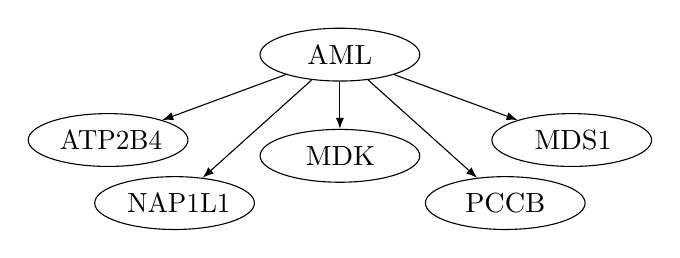
\begin{tikzpicture}[
      node distance=0.6cm and 1.5cm,
      mynode/.style={draw,ellipse,text width=1.2cm,align=center}
    ]
        \node[mynode] (y) {AML};
        \node[mynode, below=of y] (a3) {MDK};
        \node[mynode, below left=of y] (a1) {ATP2B4};
        \node[mynode, below right=of a1, right of=a3] (a2) {PCCB};
        \node[mynode, below right=of y] (a5) {MDS1};
        \node[mynode, below left=of a5, left of=a3] (a4) {NAP1L1};
        \path (y) edge[-latex] (a1)
              (y) edge[-latex] (a2)
              (y) edge[-latex] (a3)
              (y) edge[-latex] (a4)
              (y) edge[-latex] (a5);
    \end{tikzpicture}
\end{center}


\begin{table}
	\centering
	\caption{Naive Bayes network's performances}
	\label{tab:naive}
	\begin{tabular}{ccccc}
    	\toprule
    	    \multicolumn{1}{c}{k} &
    		\multicolumn{1}{c}{accuracy} &
    		\multicolumn{1}{c}{recall} &
    		\multicolumn{1}{c}{precision} &
    		\multicolumn{1}{c}{f1} \\
    	\midrule
    		1   & 0.93 & 1.00 & 0.67 & 0.80 \\
    		2   & 0.80 & 1.00 & 0.63 & 0.77 \\
    		3   & 0.86 & 1.00 & 0.71 & 0.83 \\
    		4   & 0.79 & 0.86 & 0.75 & 0.80 \\
    		5   & 0.71 & 0.83 & 0.63 & 0.71 \\[2pt]
    		\hline
    		avg & 0.82 & 0.92 & 0.68 & 0.78 \Tstrut\Bstrut\\
    	\bottomrule    
	\end{tabular}
\end{table}

The network's parameters are trained using the \ac{EM} algorithm, using the same trick of putting some expirience on all possible configurations as described in section \cref{sec:npc} for NPC. \cref{tab:naive} summarises the performances of the Naive Bayes network.

\section{Results}
\label{sec:results}

NPC and greedy search-and-score algorithm showed very similar performances, with an average accuracy of $72\%$.
In both cases, recall is much higher than precision.
This means that the network tends to classify negative examples as positive.
On the other hand, it manages to correctly identify almost all positive examples.

The Naive Bayes network performed significantly better than both the networks learned with NPC and greedy search-and-score algorithms, reaching an average accuracy of $82\%$.
Also, the network results to be simpler than the learned one.

There are two main possible explanation for this results.
The first possibility is that most of the genes are independent of each other with regards to \texttt{AML}.
In this setting, the independence assumption of the Naive Bayes approach is a good approximation of the reality, so the Naive network generalizes well on real data.
The second possibility is that the training dataset was too small to learn a good structure.
The learned structures models the noise of the sample data and do not generalize properly.

\section{Conclusions}
\label{sec:conclusions}

On this learning problem, the fixed Naive Bayes structure performed significantly better than the networks learned with both NPC and Greedy search-and-score.
Naive Bayes classifiers should considered if the training set is small and thus does not contain enough information to learn a good structure.
The network structure of a Naive Bayes classifier is simpler than the structure learned from the data and may perform better in some cases.
If the random variables are known to be independent on each other given the class, then the Naive Bayes approach should be preferred.


% \bibliographystyle{IEEEtran}
% \bibliography{references}

\end{document}
